\documentclass{article}

\usepackage{amsmath} % math stuff
\usepackage{amssymb} % math stuff
\usepackage{array} % equations and stuff
\usepackage{bm} % bold math
%\usepackage{caption} % suppressed table numbering; incompatible with revtex, and longtable, I think
\usepackage{comment} % comment environment
%\usepackage{enumitem} % customization of enumeration, itemize, and description
\usepackage[T1]{fontenc} % font encoding for special characters, must also use scalable font package
\usepackage[margin=0.8in]{geometry} % paper sizes and margins (but be careful not to mess up pre-defined pages)
\usepackage{graphicx} % for graphics
%\usepackage{helvet} % default font is the helvetica postscript font
\usepackage{layouts} % print units like widths
\usepackage{lipsum} % lorem ipsum filler text
\usepackage{lmodern} % scalable font?
\usepackage{longtable} % multi-page tables
\usepackage{mathrsfs} % math script font
\usepackage{mhchem} % easier chemical formula
\usepackage{microtype} % allows disabling of ligatures
%\usepackage{newcent} % new century schoolbook font
\usepackage{nicefrac}
\usepackage{parskip} % removes paragraph indentation, and adjusts paragraph skip, as well as list items
\usepackage{pdfpages} % add pdf files as pages
%\usepackage{setspace} % adjust text spacing and indents
\usepackage{siunitx} % decimal alignment
\usepackage{subfigure} % divided figures
%\usepackage{tabu} % extra table options
\usepackage{textcomp} % symbols
\usepackage{threeparttablex} % better footnotes with longtable
\usepackage{titling} % title placement
\usepackage{ulem} % strikethrough text
%\usepackage{url} % superceded by hyperref
\usepackage{verbatim} % verbatim environment
\usepackage{xcolor} % colors and color boxes
\usepackage{xspace} % commands that don't eat up white space
\usepackage{hyperref} % links and page setup; should always come last

\hypersetup{
	bookmarks=true,
	colorlinks=true,
	citecolor=blue,
	linkcolor=blue,
	urlcolor=blue,
	pdfstartview={XYZ null null 1.0} % default open view is 100%
}

\DisableLigatures[f,t]{encoding = T1} % disable ff, fi, fl, tt ligatures, without f option, it also disables -- = endash
\renewcommand{\arraystretch}{1.1} % extra vertical space in tables

% define matrix environment to allow vertical bar
\makeatletter
\renewcommand*\env@matrix[1][*\c@MaxMatrixCols c]{%
  \hskip -\arraycolsep
  \let\@ifnextchar\new@ifnextchar
  \array{#1}}
\makeatother

\delimitershortfall=0pt % matrix braces go all the way around text

\begin{document}

\pagestyle{empty} % don't number pages

% custom title
\begin{center}
{\LARGE Classic Riddler}

\vspace{0.15in}

{\Large 23 October 2020}
\end{center}


\section*{Riddle:}

Now that LeBron James and Anthony Davis have restored the Los Angeles Lakers to glory with their recent victory in the NBA Finals, suppose they decide to play a game of sudden-death, one-on-one basketball.
They'll flip a coin to see which of them has first possession, and whoever makes the first basket wins the game.

Both players have a 50 percent chance of making any shot they take.
However, Davis is the superior rebounder and will always rebound any shot that either of them misses.
Every time Davis rebounds the ball, he dribbles back to the three-point line before attempting another shot.

Before each of Davis's shot attempts, James has a probability $p$ of stealing the ball and regaining possession before Davis can get the shot off.
What value of $p$ makes this an evenly matched game of one-on-one, so that both players have an equal chance of winning \textit{before} the coin is flipped?

\section*{Solution:}

I have drawn a decision tree that demonstrates all the states and outcomes described in the riddle.
It can be seen on the following page.

The tree starts at the top with a coin flip.
Then either ``J'' (James) or  ``D'' (Davis) get possession.
The tree follows each possibility of shooting, scoring, missing, stealing, and rebounding, with the probabilities of each path labeled.
The two possible outcomes are J scoring and D scoring.

I have also labeled several states with letters ``a'' through ``f''.
These are the only states which are worth calculating.
For each state $i$, I define the probability $P_{i}$ as the probability of D winning from that state.
Equivalently, I could define the probability of J winning.
Trivially, $P_{\rm{e}}=0$ and $P_{\rm{f}}=1$.
From here, I can recursively build up the probabilities for the other states (skipping through the miss-and-rebound steps):

\[
P_{\rm{a}}=\frac{1}{2}P_{\rm{b}}+\frac{1}{2}P_{\rm{c}}
\]
\[
P_{\rm{b}}=\frac{1}{2}P_{\rm{c}}+\frac{1}{2}P_{\rm{e}}
\]
\[
P_{\rm{c}}=pP_{\rm{b}}+(1-p)P_{\rm{d}}
\]
\[
P_{\rm{d}}=\frac{1}{2}P_{\rm{c}}+\frac{1}{2}P_{\rm{f}}
\]

After plugging in the two initial values, solving these equations is equivalent to row reducing the following matrix:

\[
\begin{bmatrix}[cccc|c]
1 & -\nicefrac{1}{2} & -\nicefrac{1}{2} & 0      & 0 \\
0 & 1            & -\nicefrac{1}{2} & 0      & 0 \\
0 & -p           & 1            & -(1-p) & 0 \\
0 & 0            & -\nicefrac{1}{2} & 1      & \nicefrac{1}{2}
\end{bmatrix}
\]

This gives the solutions

\[
P_{\rm{a}}=\frac{3(1-p)}{4}
\]
\[
P_{\rm{b}}=\frac{1-p}{2}
\]
\[
P_{\rm{c}}=1-p
\]
\[
P_{\rm{d}}=\frac{2-p}{2}
\]

If the probability of both players winning is equal from the coin toss, then $P_{\rm{a}}=\nicefrac{1}{2}$.
This gives the solution $p=\nicefrac{1}{3}$.
As a manual check, plugging this in to the above equations is correct.
So the solution is
\fcolorbox{red}{white}{$\bm{{p=\nicefrac{1}{3}}}$}\,.


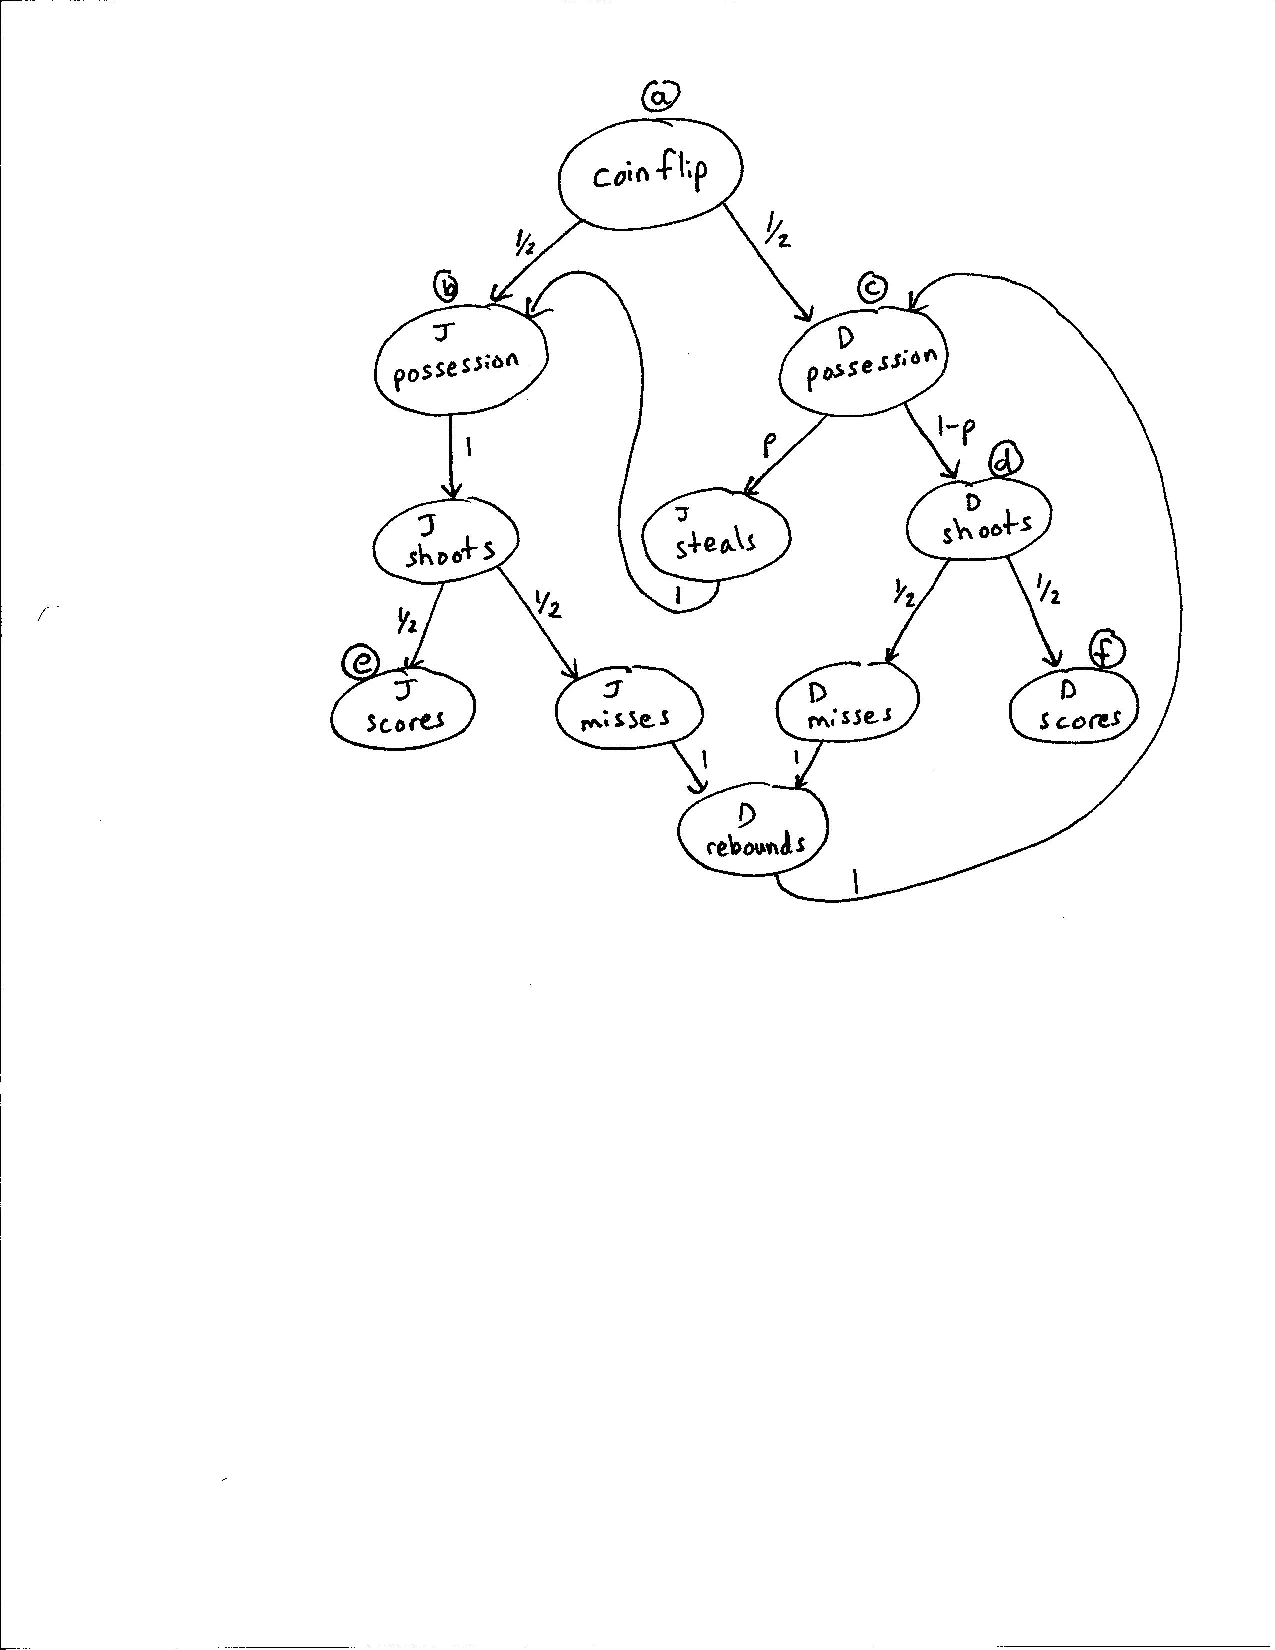
\includepdf{Tree.pdf}



\end{document}